\documentclass{article}

\usepackage{amsmath,amssymb}
\usepackage{tikz}
\usepackage{pgfplots}
\usepackage{xcolor}
\usepackage[left=2.1cm,right=3.1cm,bottom=3cm,footskip=0.75cm,headsep=0.5cm]{geometry}
\usepackage{enumerate}
\usepackage{enumitem}
\usepackage{marvosym}
\usepackage{tabularx}
\usepackage{multirow}

\usepackage[utf8]{inputenc}

\renewcommand*{\arraystretch}{1.4}

\newcolumntype{L}[1]{>{\raggedright\arraybackslash}p{#1}}
\newcolumntype{R}[1]{>{\raggedleft\arraybackslash}p{#1}}
\newcolumntype{C}[1]{>{\centering\let\newline\\\arraybackslash\hspace{0pt}}m{#1}}

\title{\textbf{Rechtfertigung der Staatstätigkeit, Hausaufgabe 4}}
\author{\textsc{Henry Haustein}}
\date{}

\begin{document}
	\maketitle
	
	\section*{Aufgabe 2}
	\begin{enumerate}[label=(\alph*)]
		\item Die privaten Grenzkosten sind $GK^{priv}=2x$. Die sozialen Grenzkosten sind $GK^{soz}=GK^{priv} + GS = 2x + 20$. Die optimale Menge ist bei
		\begin{align}
			GK^{soz} &= p \notag \\
			2x^{opt} + 20 &= 50 \notag \\
			x^{opt} &= 15 \notag
		\end{align}
		Ohne staatlichen Eingriff wird
		\begin{align}
			GK^{priv} &= p \notag \\
			2x^{priv} &= 50 \notag \\
			x^{priv} &= 25 \notag
		\end{align}
		hergestellt.
		\item Der Wohlfahrtsverlust ist
		\begin{align}
			\frac{1}{2}(x^{priv} - x^{opt}) \cdot GS = \frac{1}{2}(25-15)\cdot 20 = 100 \notag
		\end{align}
		\item Diagramm
		\begin{center}
			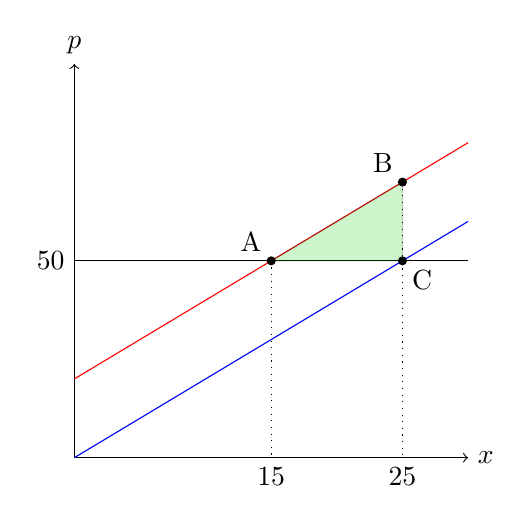
\begin{tikzpicture}
				\draw[->] (0,0) -- (5,0) node[right] {$x$};
				\draw[->] (0,0) -- (0,5) node[above] {$p$};
				
				\draw (0,2.5) node[left] {50} -- (5,2.5);
				\draw[blue] (0,0) -- (5,3);
				\draw[red] (0,1) -- (5,4);
				
				\draw[dotted] (4.167,3.5) -- (4.167,0) node[below] {25};
				\draw[dotted] (2.5,2.5) -- (2.5,0) node[below] {15};
				
				\draw[fill=green!80!black,opacity=0.2] (2.5,2.5) -- (4.167,3.5) -- (4.167,2.5) -- (2.5,2.5);
				
				\draw[fill=black] (4.167,2.5) circle (0.05) node[below right] {C};
				\draw[fill=black] (2.5,2.5) circle (0.05) node[above left] {A};
				\draw[fill=black] (4.167,3.5) circle (0.05) node[above left] {B};
			\end{tikzpicture} \\
			\textcolor{blue}{$GK^{priv}$}, \textcolor{red}{$GK^{soz}$}, \textcolor{green!80!black}{Wohlfahrtsverlust}
		\end{center}
		\item Die Pigou-Steuer soll die Kosten des Umweltschadens in $x^{opt}$ darstellen, also
		\begin{align}
			t &= GK^{soz}(x^{opt}) - GK^{priv}(x^{opt}) \notag \\
			&= (2\cdot 15+20) - (2\cdot 15) \notag \\
			&= 20 \notag
		\end{align}
		Das Steueraufkommen beträgt dann $x^{opt}\cdot t = 15\cdot 20 = 300$.
	\end{enumerate}
	
	\section*{Aufgabe 3}
	\begin{enumerate}[label=(\alph*)]
		\item Es gilt
		\begin{align}
			\begin{array}{lcl}
				GV_1 = 60-s_1 & \Rightarrow & s_1 = 60-GV_1 \\
				GV_2 = 60-2s_2 & \Rightarrow & s_2 = 30 - \frac{1}{2}GV_2 \\
				\cline{3-3}
				&&s\;\, = 90 - \frac{3}{2}GV
			\end{array} \notag
		\end{align}
		Also $GV = 60 - \frac{2}{3}s$.
		\item Es gilt
		\begin{align}
			\begin{array}{lcl}
				D_1 = \frac{1}{2}s_1^2 & \Rightarrow & GD_1 = s_1 \\
				D_2 = \frac{1}{2}s_2^2 & \Rightarrow & GD_2 = s_2 \\
				\cline{3-3}
				&&GD\;\, = 2s
			\end{array} \notag
		\end{align}
		\item Die Unternehmen kaufen solange ein, bis $GV=p$, also
		\begin{align}
			GV &= p \notag \\
			60-\frac{2}{3}s^{priv} &= 4 \notag \\
			s^{priv} &= 84 \notag
		\end{align}
		\item Mit der Samuelson-Regel folgt
		\begin{align}
			\sum GV_i &= \sum GN_j \notag \\
			GV &= GD \notag \\
			60-\frac{2}{3}s^{opt} &= 2s^{opt} \notag \\
			s^{opt} &= 22.5 \notag
		\end{align}
		\item Die Pigou-Steuer soll die Grenznachteile bei $s^{opt}$ aufwiegen, also
		\begin{align}
			t = GD(s^{opt}) = 2\cdot 22.5 = 45 \notag
		\end{align}
		\item Die Unternehmen teilen sich $s^{opt}$ so auf, dass $GV_1=GV_2$ unter der Nebenbedingung $s_1+s_2=22.5$ gilt:
		\begin{align}
			GV_1 &= GV_2 \notag \\
			60-s_1 &= 60-2\cdot (22.5-s_1) \notag \\
			s_1 &= 15 \notag \\
			s_2 &= 7.5 \notag
		\end{align}
	\end{enumerate}

\end{document}